% A Lopsided Victory — generated from src/chapters/02-lopsided/index.svx by scripts/print.mjs.
% Do not edit: changes here are overwritten on the next export.

\chapter{A Lopsided Victory}
\label{ch:lopsided}

\section{Show Me the Money}

\lettrine{I}{} once volunteered for a career day event at my daughter’s middle school. Like the other volunteers, my role was to occupy a seat at a table in the cafeteria, on top of which sat a sign with the name of my occupation, \emph{Data Scientist}, printed on it. Kids could stop by and talk to me about my profession and ask questions about what kinds of tasks it involves, what a typical day is like, and more. One young man, who seemed genuinely intrigued by my explanation of the work of a data scientist, seemed conflicted after our brief chat.

“I’ve always wanted to be a CEO, but your job \emph{does} sound really cool,” he remarked.

“What is it about being a CEO that appeals to you?” I asked.

“They get to be in charge, and they make a \emph{lot} of money!” he responded frankly. He didn’t know exactly how much he could expect to earn as a CEO, but he was sure that it was significantly more than most people who worked ordinary jobs.

For many people, expected earnings are a very important factor in deciding between careers or jobs. Wages, however, are not normally distributed, which creates challenges when comparing earnings statistics for two occupations. The Bureau of Labor Statistics regularly publishes wage data for standard occupational classifications, and if we use our checklist from Chapter 1, we can evaluate the process that generates these data and determine how likely they are to follow a bell curve.

First, an individual’s pay at a given point in time is shaped by dozens of factors, including their level of education, experience, geographic location, the industry in which they work, any licenses or specialized credentials they may hold, unique skills they may possess, and more. As a result, the process that generates wage data passes our \emph{many pieces} test.

The second test, for additivity, fails quite clearly. Pay raises are frequently calculated as a percentage, so a 4\% raise is worth far more in dollars to someone earning a high salary than to someone earning a lower one. Premiums for rare credentials or a particular geography, like a big city, also behave approximately like multipliers, and this again violates our second item on the checklist.

The independence test holds only partially. Workers with high levels of education are more likely to hold specialized credentials and licenses, high-paying industries are more likely to cluster in big cities, and rare skills are more likely to come with more experience. In essence, many of the pieces we outlined in the first test tend to move together, violating the requirement for independence. When this occurs, an individual’s advantages tend to accumulate rather than averaging out, which increases the spread across salary levels.

The \emph{no giants} test mostly passes, although occupations in which bonuses and commissions make up a large portion of a particular year’s pay may violate this.

Finally, the one-group test partially fails since certain occupational categories are much more heterogeneous than others. For example, \emph{General and operations managers} is a broad occupational category that encompasses a fairly wide range of management jobs, while \emph{Data scientists} tends to be a much narrower classification.

Here’s what our completed checklist might look like for salary data by occupation:

\begin{bookfigure}
	\caption{Field Guide 1.1, Applied to Wages}\label{fig:wage-checklist}
	\begin{appliedguide}
		\guidesection{How each value is built}
		\guideverdict{pass}{Many pieces}{Education, experience, location, industry, credentials, and skills all shape pay.}
		\guideverdict{fail}{Additive}{Raises and pay premiums are percentages, so they multiply rather than add.}
		\guideverdict{partly}{Independent}{Education, credentials, location, and experience tend to travel together.}
		\guideverdict{partly}{No giants}{Mostly small pieces, but bonuses and commissions can dominate a year’s pay.}
		\guidesection{Whether the values belong together}
		\guideverdict{partly}{One group}{Broad job titles, like general and operations managers, mix very different jobs.}
		\guidepara{\emph{Verdict:} don’t expect a bell. Expect a curve that leans to the right, as in Figure~\ref{fig:salaries}.}
	\end{appliedguide}
\end{bookfigure}

The test that fails most clearly is the one for additivity, and when this particular test fails, it tends to stretch the distribution to one side. Understanding why is fairly straightforward if we conduct a simple thought experiment: imagine two individuals, each earning \$100,000 per year. If the first individual doubles their salary twice (doubling is \emph{multiplying} by two), they end up at \$400,000. If the second individual halves their salary twice (dividing by two is the same as multiplying by one-half), they end up at \$25,000. The process is bounded at zero for the poor worker whose salary keeps halving, but the sky’s the limit for the lucky one who keeps experiencing a doubling of their salary. This multiplicative process leads to right-skewed distributions with long tails, like the ones we see in Figure~\ref{fig:salaries}.

\begin{bookfigure}
	\caption{Managers Earn More on Average; Data Scientists Earn More Typically}\label{fig:salaries}
	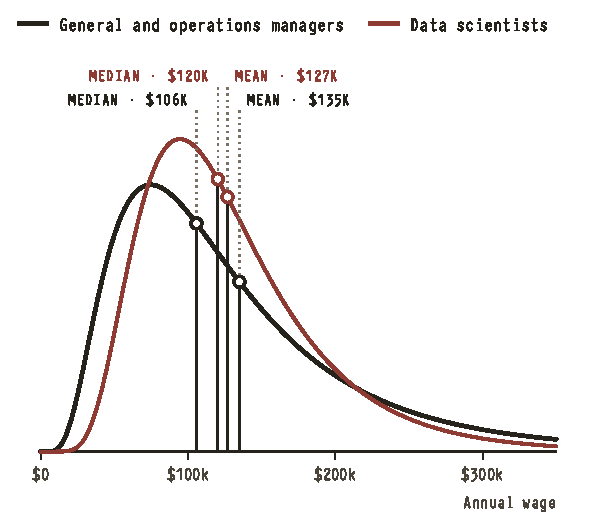
\includegraphics[width=\textwidth]{figures/2-2-salaries.pdf}
	\figurenote{Bureau of Labor Statistics, Occupational Employment and Wage Statistics, May 2025}{Curves are lognormal shapes fitted to each occupation’s published 25th and 75th percentile wages; each falls within about 5\% of the published 10th, 50th, and 90th percentiles and within about 2\% of the published mean. Markers show the published mean and median, colored by occupation}
\end{bookfigure}

In this figure we see two wage distributions: one for the \emph{General and operations managers} occupational category, and another for \emph{Data scientists.} While this particular class of managers is below the level that the young man from the career day event aspired to, it’s plausible that he may consider this occupational category some day. If he just looked at the mean salaries, he would conclude that workers in the manager classification earn more money than data scientists. However, the median values tell a different story. Half of all data scientists are estimated to earn at least \$120,000, while the corresponding figure for general and operations managers is just \$106,000.

\section{Playing the Game}

So which figure should we trust if our goal is to understand how much we can expect to earn in one occupation versus the other? Notice that the two lines in the plot cross at two points --- once around the \$73,000 mark, and again near \$214,000. We can think of our pay scale as being partitioned into three sections with the boundaries at those very points. Looking at it this way, we see that data scientist salaries are more concentrated in the middle section, while manager salaries are more concentrated at the ends. That is to say, managers are more likely to earn low salaries while also being more likely to earn very high salaries.

Comparing these kinds of distributions leaves the prospective worker in a situation that may feel somewhat like a game of chance. Imagine, for example, two booths at the county fair: at Booth A, everyone is guaranteed to win \$100, and at Booth B, there’s a 90\% chance you win \$95 and a 10\% chance that you win \$250. The average, or expected value, of Booth B’s winnings is \$110.50 (\(0.9 \times 95 + 0.1 \times 250\)) and the median payout is simply \$95. At Booth A, both the expected and median values are \$100. This means that Booth B will pay out more than Booth A \emph{on average}, but nine out of every ten players at Booth B will end up worse off than they would have been had they instead chosen to play at Booth A. However, the law of large numbers tells us that the average winnings of those who play at Booth B over and over again will eventually approach \$110.50. Nonetheless, that provides little comfort to someone choosing between careers because, as we all know, we only get to play the game of life once! In the case of our two wage distributions, the data scientist wage distribution is analogous to Booth A and general and operations managers are analogous to Booth B.

This exercise shows us that for certain distributions, comparisons require more nuance than simply checking a single measurement from each distribution. The larger mean combined with the lower median for the managers distribution provided a clue that it had a longer and fatter tail than that of the data scientists distribution, and the lower median from the managers distribution indicated that the typical manager earns less than the typical data scientist. Comparing the whole distributions made the picture very clear as it allowed us to see that managers’ salaries are spread out more than data scientists’ salaries.

We should also remind ourselves that salaries aren’t random --- for a student deciding on a career, their salary won’t be a random draw from the applicable salary distribution. Instead, it will be determined by the multitude of factors that we covered as we worked through the checklist. Even though a manager is more than twice as likely as a data scientist to earn less than \$60,000, that’s likely a result of the heterogeneity across the occupations within this particular occupational category. If the young man from the career day event obtains the right credentials and experience, and finds employment in a large city, for example, it would be reasonable for him to disregard the lower end of both of these distributions and instead focus on the higher end.

\section{Log Houses}

House prices are another example of a right-skewed distribution. Let’s once again work through our checklist to understand why this is the case:

\begin{bookfigure}
	\caption{Field Guide 1.1, Applied to Home Values}\label{fig:housing-checklist}
	\begin{appliedguide}
		\guidesection{How each value is built}
		\guideverdict{pass}{Many pieces}{Location, size, lot, age, condition, schools, and views all shape a home’s value.}
		\guideverdict{fail}{Additive}{Location and appreciation work as multipliers: the same house costs several times more in one city than another, and prices grow by percentages.}
		\guideverdict{partly}{Independent}{Big houses tend to be built on big lots, and condition is generally related to age.}
		\guideverdict{partly}{No giants}{In expensive cities, the land under a house can be worth more than the house itself.}
		\guidesection{Whether the values belong together}
		\guideverdict{fail}{One group}{Nationwide data mix housing markets as different as rural Mississippi and San Jose.}
		\guidepara{\emph{Verdict:} don’t expect a bell. Expect a curve with a long right tail, as in Figure~\ref{fig:home-values}.}
	\end{appliedguide}
\end{bookfigure}

The U.S. Census Bureau’s American Community Survey (ACS) is conducted annually and covers approximately 3.5 million addresses across the United States and Puerto Rico. Respondents are asked about where they live and what the value of their home is. Using the data for 2024, the mean home value for single-family, detached houses was \$501,000, the median was \$350,000, and the mode was \$268,000. This pattern, \(\text{mode} < \text{median} < \text{mean}\), tells us that we are dealing with a right-skewed distribution. Figure 2.4 shows an estimate of the probability density for home values, as reported by ACS respondents:

\begin{bookfigure}
	\caption{Home Values: A Long Tail to the Right}\label{fig:home-values}
	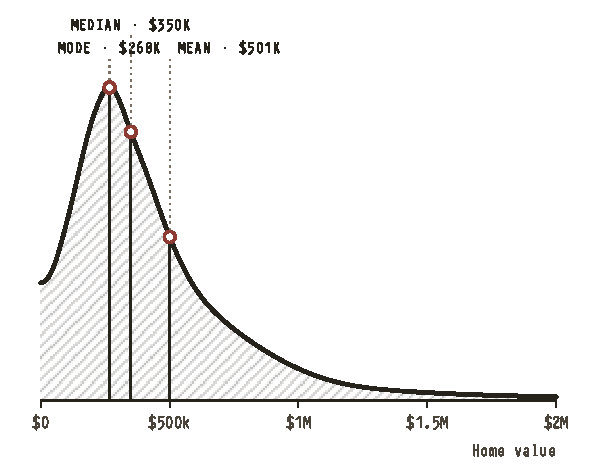
\includegraphics[width=\textwidth]{figures/2-4-home-values.pdf}
	\figurenote{U.S. Census Bureau, American Community Survey 1-year microdata, 2024}{Owner-occupied single-family detached homes, valued by their owners. About 2\% of homes are worth more than \$2 million and extend off the right edge}
\end{bookfigure}

We now know that the multiplicative effects of location and appreciation, at least in part, are responsible for the long tail we see in the plot. Just as we saw with the net worth distribution in Chapter 1, the horizontal axis in this plot is truncated because we are using a linear scale and cutting it short is necessary to produce a readable chart. However, if we simply change the scale of our x-axis, something very interesting happens, as you can see in Figure 2.5:

\begin{bookfigure}
	\caption{On a Log Scale, the Bell Comes Back (Mostly)}\label{fig:home-values-log}
	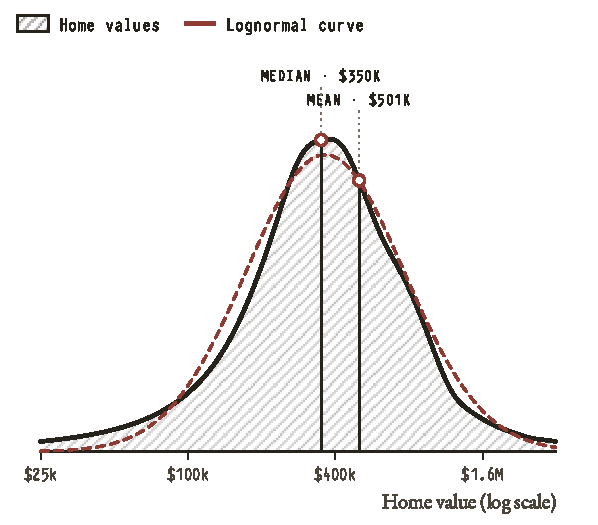
\includegraphics[width=\textwidth]{figures/2-5-home-values-log.pdf}
	\figurenote{U.S. Census Bureau, American Community Survey 1-year microdata, 2024}{Each step along the axis multiplies the value rather than adding to it. The dashed lognormal curve is fitted to the 25th and 75th percentiles. About 2\% of homes are worth less than \$25,000 and 1\% more than \$3.2 million}
\end{bookfigure}

By simply shifting from a linear scale to a logarithmic one, our home values data bunch up into a rough bell shape. Notice in Figure 2.4 that each increment on the x-axis is an increase in value of \$200,000, but in Figure 2.5, each increment represents a 4x increase in value --- this is the log transform in action. When a distribution forms a bell curve on a log scale, it is simply known as a \emph{lognormal} distribution, and many processes follow this kind of distribution. Everything from asset prices, incomes, and firm sizes, to rainfall, network response times, and viral loads have been shown to follow a lognormal distribution.

So how does this help us in practice? Let’s consider more home value data. This time, we’ll look at the distributions for two different states, and we’ll see how the log transformation, along with a few tweaks in how we think about and describe the data, helps us perform a better analysis.

Figure 2.6 shows estimates of the probability densities for home values in Wisconsin, compared to Massachusetts, again on a log scale.

\begin{bookfigure}
	\caption{Same Shape, Twice the Price}\label{fig:state-pair}
	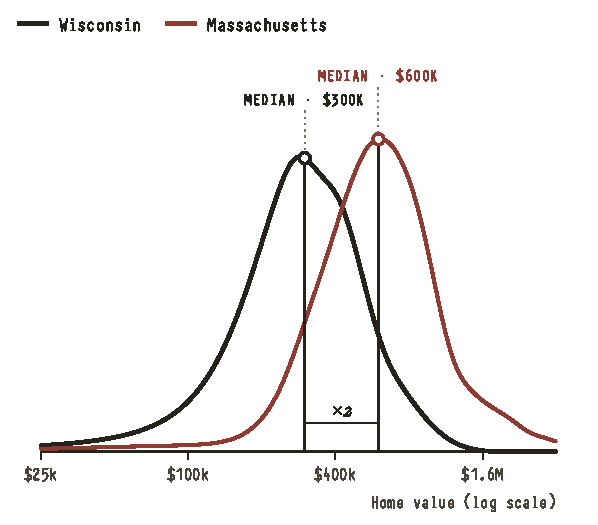
\includegraphics[width=\textwidth]{figures/2-6-state-pair.pdf}
	\figurenote{U.S. Census Bureau, American Community Survey 1-year microdata, 2024}{Owner-occupied single-family detached homes, valued by their owners. The Census Bureau reports the highest values in each state (just under 1\% of homes) only as above a cap, so the curves leave them out}
\end{bookfigure}

We can see from this plot that the shape of the distributions on the log scale is strikingly similar, just shifted. Remembering that our log axis is effectively a multiplicative scale, this allows us to compare the two markets with a single value, just stated as a multiple. In fact, home values in Massachusetts are roughly two times home values in Wisconsin, across their respective distributions. Table 2.1 demonstrates this:

\begin{booktable}
	\caption{Home Values in Wisconsin and Massachusetts}\label{tab:state-pair-table}
	\begin{tabular*}{\linewidth}{@{}l@{\extracolsep{\fill}}rrrrrr@{}}
		\toprule
		\tablehead{State} & \tablehead{10th} & \tablehead{25th} & \tablehead{Median} & \tablehead{75th} & \tablehead{90th} & \tablehead{Mean} \\
		\midrule
		Wisconsin & \$125K & \$200K & \$300K & \$420K & \$600K & \$350K \\
		Massachusetts & \$300K & \$415K & \$600K & \$850K & \$1.2M & \$740K \\
		\midrule
		\textit{Ratio} & \textit{2.4×} & \textit{2.1×} & \textit{2.0×} & \textit{2.0×} & \textit{2.0×} & \textit{2.1×} \\
		\bottomrule
	\end{tabular*}
	\figurenote{U.S. Census Bureau, American Community Survey 1-year microdata, 2024}{Percentiles and means of owner-reported values for owner-occupied single-family detached homes. The ratio is Massachusetts ÷ Wisconsin}
\end{booktable}
